\chapter{Data Transmitting and Platforms} \label{ch:platform}
The statistic data collected by a doorway counter is not of much use until it is analyzed. For a quick acquisition of data and a frequently updated overview of room occupancy, the count value should be sent to a remote platform at every time for further visualization and analyse.
\section{MQTT protocol}
We use MQTT (message queuing telemetry transport) to transfer data because it is supported by the ESP-IDF and widely accepted in IoT use cases. MQTT is an application layer protocol built on top of Wifi and TCP/IP. It is a light-weight, publish-subscribe network protocol, its structure is shown in \autoref{fig:mqtt}. When a publisher publishes, instead of sending to the receiver directly, the message is sent to a intermediate server called broker. Each message is published to a specific topic, a client would filter the messages by the subscribed topic and could only receive the message if it is listening to the same topic.

The light-weight usage of MQTT is mainly reflected by its transparent topic mechanism. A client does not need to create a topic before it publish or subscribe to it. A topic keeps alive when there is at least one publisher or subscriber. When a topic has at least one client on both pub/sub side, the data transmission becomes valid almost immediately. The topics in MQTT decouple the rigid connection between clients, reducing the complexity of connection drastically regardless of the scale (up to tens of thousands per MQTT server).

The main drawback of MQTT is no message buffering. A QoS (Quality of Service) setting higher than 0 on the client side only confirms that the message is received by the broker. If a message is published to a topic without listeners, that message is lost forever. Latest versions of MQTT supports retained messages, which stores one \emph{last known good value} in the broker. However, the retained messages aim to serve as a \emph{initialization default value} for those subscriber that join the topic between two publish intervals, storing more than one message is impossible. Secondly, MQTT is a queuing system instead of streaming, it delivers messages to a single consumer. When there are multiple consumers subscribing to a topic, they will consume the messages in a round-robin manner.
\begin{figure}
  \centering
  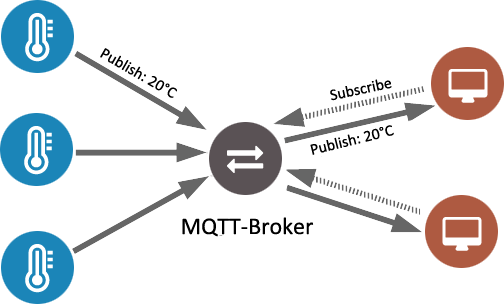
\includegraphics[width=0.6\textwidth]{figures/mqtt.png}
  \caption{MQTT network structure}\label{fig:mqtt}
\end{figure}
\section{Node-Red}
\begin{figure}
  \centering
  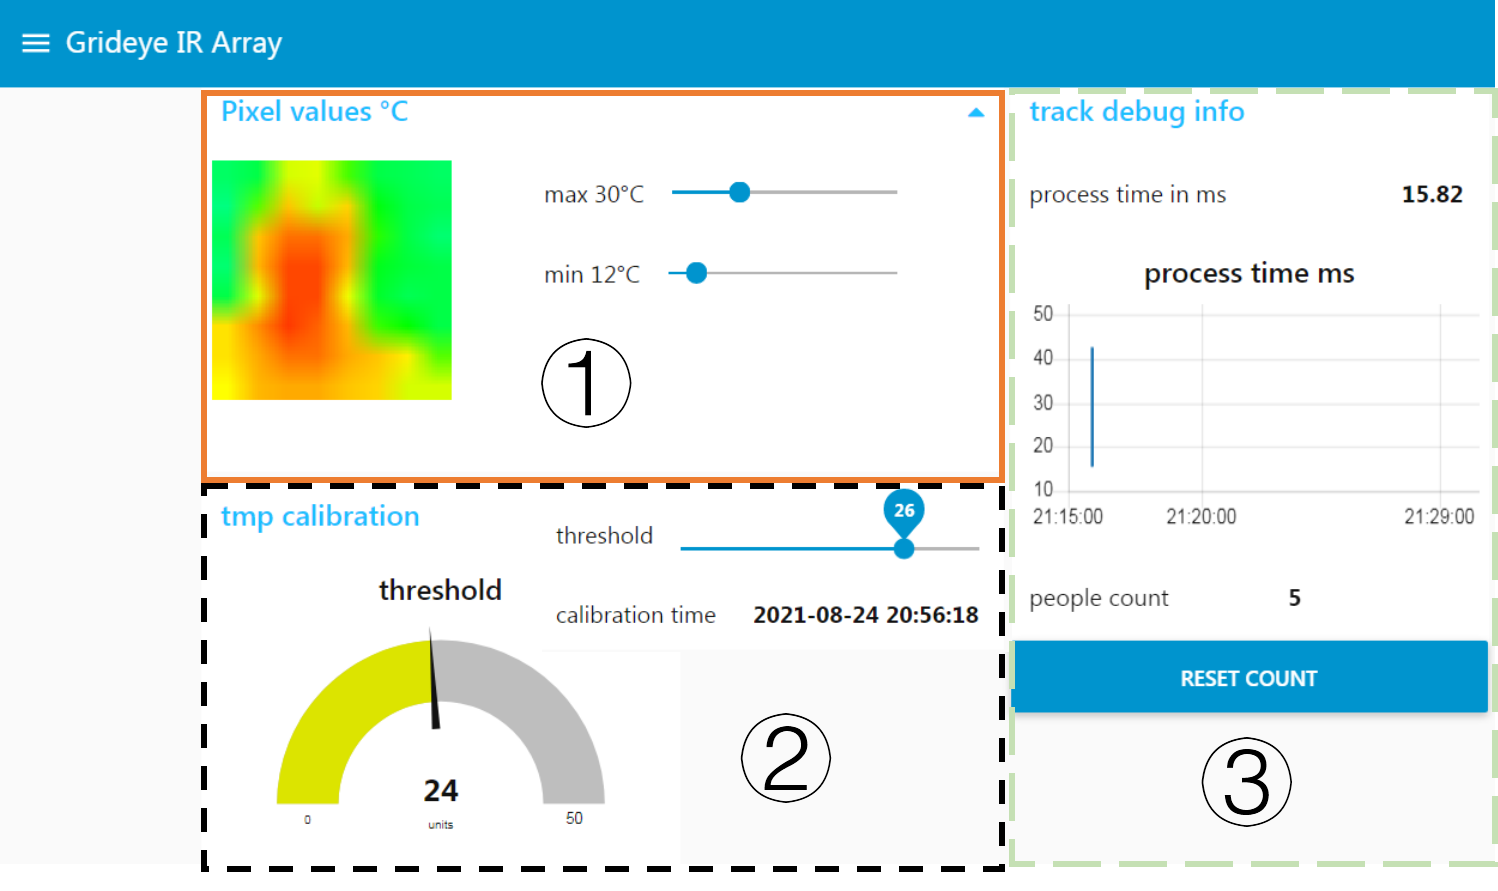
\includegraphics[width=0.8\textwidth]{figures/noderedui.png}
  \caption{Our NodeRed visualization panel is divided into three sections: (1)raw image frame, (2)temperature sensor reading, (3)debug info}\label{fig:nodered}
\end{figure}

Visualization of an image frame sequence on websites often requires extensive programming. Fortunately, Node-Red \cite{nodered} relieves us from irrelevant affairs so that we can concentrate on the doorway counter development. Node-Red is a web-based visual programming editor that connects IoT devices or acts as an end-consumer. The smallest execution unit is called a node.
%todo: overview of network dataflow
%
\section{ElasticSearch and Kibana} 